\documentclass[aspectratio=169, 10pt]{beamer}

% --- GÓI HỌC THUẬT & FONT TIẾNG VIỆT CHO XELATEX ---
\usepackage{fontspec}
\setmainfont{Arial}
\setsansfont{Arial}
\setmonofont{Consolas}

\usepackage{amsmath,amssymb}
\usepackage{graphicx}
\usepackage{booktabs}
\usepackage{tabularx}
\usepackage{multicol}
\usepackage{listings}
\usepackage{xcolor}
\usepackage{tikz}
\usetikzlibrary{shapes,arrows,positioning,fit,backgrounds,calc}
\usepackage{tcolorbox}
\tcbuselibrary{skins,breakable,listings}

% --- ĐỊNH NGHĨA MÀU SẮC CHUẨN ĐẠI HỌC & C# .NET ---
\definecolor{UniNavy}{RGB}{15, 44, 89}        % Xanh hải quân chủ đạo (#0F2C59)
\definecolor{UniBlue}{RGB}{29, 93, 155}       % Xanh Slate (#1D5D9B)
\definecolor{CSharpPurple}{RGB}{104, 33, 122} % Tím nhận diện C# & Visual Studio (#68217A)
\definecolor{UniLightBlue}{RGB}{232, 241, 252}% Nền xanh nhạt
\definecolor{UniOrange}{RGB}{225, 112, 18}    % Cam nhấn mạnh (#E17012)
\definecolor{UniGreen}{RGB}{30, 132, 73}      % Xanh lá thực hành (#1E8449)
\definecolor{UniDark}{RGB}{33, 37, 41}        % Màu chữ chính / nền console
\definecolor{CodeBg}{RGB}{248, 249, 250}      % Nền code
\definecolor{CSharpKeyword}{RGB}{0, 0, 255}   % Xanh dương từ khóa C#
\definecolor{CSharpString}{RGB}{163, 21, 21}  % Đỏ chuỗi C#
\definecolor{CSharpComment}{RGB}{0, 128, 0}   % Xanh lá chú thích C#

% --- CẤU HÌNH THEME BEAMER MADRID WIDESCREEN ---
\usetheme{Madrid}
\usecolortheme{whale}

\setbeamercolor{palette primary}{bg=UniNavy, fg=white}
\setbeamercolor{palette secondary}{bg=CSharpPurple, fg=white}
\setbeamercolor{palette tertiary}{bg=UniNavy!85, fg=white}
\setbeamercolor{palette quaternary}{bg=UniNavy, fg=white}

\setbeamercolor{structure}{fg=UniNavy}
\setbeamercolor{titlelike}{parent=structure, fg=UniNavy}
\setbeamercolor{frametitle}{bg=UniNavy, fg=white}
\setbeamercolor{frametitle continuation}{fg=white}
\setbeamercolor{normal text}{fg=UniDark}

% Cấu hình khối thông tin (Blocks)
\setbeamercolor{block title}{bg=UniBlue, fg=white}
\setbeamercolor{block body}{bg=UniLightBlue!40, fg=UniDark}
\setbeamercolor{block title example}{bg=UniGreen, fg=white}
\setbeamercolor{block body example}{bg=UniGreen!10, fg=UniDark}
\setbeamercolor{block title alerted}{bg=UniOrange, fg=white}
\setbeamercolor{block body alerted}{bg=UniOrange!10, fg=UniDark}

% Cấu hình Footline chuyên nghiệp
\setbeamertemplate{navigation symbols}{}
\setbeamertemplate{footline}{
  \leavevmode%
  \hbox{%
    \begin{beamercolorbox}[wd=.35\paperwidth,ht=2.5ex,dp=1.1ex,left,leftskip=2ex]{author in head/foot}%
      \usebeamerfont{author in head/foot}\textbf{Lớp IT26M} | Lập trình C\# \& .NET
    \end{beamercolorbox}%
    \begin{beamercolorbox}[wd=.45\paperwidth,ht=2.5ex,dp=1.1ex,center]{title in head/foot}%
      \usebeamerfont{title in head/foot}Chương 4: Lớp, Đối tượng, Phương thức và Chuỗi
    \end{beamercolorbox}%
    \begin{beamercolorbox}[wd=.20\paperwidth,ht=2.5ex,dp=1.1ex,right,rightskip=2ex]{date in head/foot}%
      \usebeamerfont{date in head/foot}\insertframenumber{} / \inserttotalframenumber
    \end{beamercolorbox}%
  }%
  \vskip0pt%
}

% --- CẤU HÌNH GÓI LISTINGS CHO C# & TERMINAL ---
\lstdefinelanguage{CSharpCustom}{
  keywords={abstract, as, base, bool, break, byte, case, catch, char, checked, class, const, continue, decimal, default, delegate, do, double, else, enum, event, explicit, extern, false, finally, fixed, float, for, foreach, goto, if, implicit, in, int, interface, internal, is, lock, long, namespace, new, null, object, operator, out, override, params, private, protected, public, readonly, ref, return, sbyte, sealed, short, sizeof, stackalloc, static, string, struct, switch, this, throw, true, try, typeof, uint, ulong, unchecked, unsafe, ushort, using, virtual, void, volatile, while, async, await, var, get, set, value},
  keywordstyle=\color{CSharpKeyword}\bfseries,
  ndkeywords={Console, String, Math, Convert, int, double, float, char, bool, decimal, Account, AccountTest},
  ndkeywordstyle=\color{CSharpPurple}\bfseries,
  sensitive=true,
  comment=[l]{//},
  morecomment=[s]{/*}{*/},
  commentstyle=\color{CSharpComment}\itshape,
  stringstyle=\color{CSharpString},
  morestring=[b]",
  morestring=[b]'
}

\lstset{
  language=CSharpCustom,
  basicstyle=\ttfamily\scriptsize,
  backgroundcolor=\color{CodeBg},
  frame=single,
  rulecolor=\color{gray!30},
  breaklines=true,
  breakatwhitespace=true,
  tabsize=2,
  showstringspaces=false,
  numbers=left,
  numberstyle=\tiny\color{gray},
  numbersep=5pt,
  xleftmargin=12pt,
  framexleftmargin=10pt
}

% Style cho console output
\lstdefinestyle{terminalStyle}{
  basicstyle=\ttfamily\scriptsize\color{white},
  backgroundcolor=\color{UniDark},
  frame=single,
  rulecolor=\color{UniNavy},
  numbers=none,
  xleftmargin=6pt,
  framexleftmargin=6pt
}

% --- THÔNG TIN TRANG TIÊU ĐỀ ---
\title[\textbf{Lập trình C\# \& .NET -- Chương 4}]{\textbf{\LARGE KỸ THUẬT LẬP TRÌNH C\#}}
\subtitle{\textbf{\large Chương 4: Lớp, Đối tượng, Phương thức và Chuỗi\\(Introduction to Classes, Objects, Methods and strings)}}
\author[\textbf{Khoa CNTT -- IT26M}]{\textbf{BÀI GIẢNG CHUẨN ĐẠI HỌC (3 TIẾT TÍCH HỢP)}\\Giáo trình: \textit{Visual C\# How to Program} (Deitel \& Deitel)}
\institute[\textbf{Lớp IT26M}]{\textbf{Khoa Công nghệ Thông tin -- Đại học Đông Á}\\\textbf{Đối tượng:} Lớp IT26M (Khóa 2026)}
\date[\textbf{2026}]{\textbf{Học kỳ I -- Năm học 2026}}

\begin{document}

% ==============================================================================
% SLIDE 1: TRANG TIÊU ĐỀ BÀI GIẢNG
% ==============================================================================
\begin{frame}[plain]
  \titlepage
  \begin{center}
    \scriptsize \color{gray} Bản quyền bài giảng thuộc Bộ môn Kỹ thuật Lập trình -- Phục vụ đào tạo Đại học chính quy
  \end{center}
\end{frame}

% ==============================================================================
% SLIDE 2: MỤC TIÊU BÀI HỌC & CHUẨN ĐẦU RA (CLOs)
% ==============================================================================
\begin{frame}{Mục tiêu Bài học \& Chuẩn đầu ra (CLOs)}
  \begin{block}{\textbf{Chuẩn đầu ra sinh viên cần đạt được sau buổi học 3 tiết:}}
    \begin{itemize}
      \item \textbf{CLO 4.1 (Understand):} Phân biệt \textbf{Lớp} (Class), \textbf{Đối tượng} (Object), \textbf{Driver Class} (\texttt{Main}), \textbf{Kiểu tham chiếu} vs \textbf{Kiểu giá trị}, toán tử \texttt{new} và giá trị mặc định \texttt{null}.
      \item \textbf{CLO 4.2 (Apply):} Khai báo phương thức, phân biệt \textbf{Tham số} vs \textbf{Đối số}, \textbf{Biến thể hiện} (Instance Variables) vs \textbf{Biến cục bộ}, thiết lập \texttt{private} để \textbf{Đóng gói} (Encapsulation).
      \item \textbf{CLO 4.3 (Apply):} Xây dựng \textbf{Thuộc tính} (Properties) với \texttt{get}/\texttt{set}, từ khóa \texttt{value}, vận dụng \textbf{Auto-Implemented Properties} (\texttt{\{ get; set; \}}) và đọc \textbf{Sơ đồ lớp UML}.
      \item \textbf{CLO 4.4 (Apply):} Khởi tạo đối tượng bằng \textbf{Hàm tạo} (Constructors), phân biệt hàm tạo mặc định vs tùy biến, quy tắc nạp chồng và quản lý vùng nhớ Heap.
      \item \textbf{CLO 4.5 (Create):} Vận dụng kiểu \texttt{decimal} (128-bit, hậu tố \texttt{m}), xây dựng cơ chế \textbf{Kiểm tra tính hợp lệ} (Data Validation), định dạng tiền tệ \texttt{:C} cho ứng dụng tài khoản ngân hàng.
    \end{itemize}
  \end{block}
  \vspace{-2mm}
  \begin{exampleblock}{\textbf{Phương pháp sư phạm:}}
    Học qua dự án thực tế (\textit{Case-Based Learning}): Xây dựng và hoàn thiện lớp quản lý tài khoản ngân hàng \textbf{Account} qua các bước nâng cấp từ đơn giản đến chuyên nghiệp!
  \end{exampleblock}
\end{frame}

% ==============================================================================
% SLIDE 3: TIẾN TRÌNH BÀI HỌC 3 TIẾT
% ==============================================================================
\begin{frame}{Tiến trình Bài học 3 Tiết (150 Phút Tích hợp)}
  \begin{columns}[T]
    \begin{column}{0.32\textwidth}
      \begin{tcolorbox}[colback=UniNavy!10,colframe=UniNavy,title=\textbf{TIẾT 1 (50')},fonttitle=\small\bfseries]
        \textbf{Lớp, Đối tượng \& Set/Get}
        \begin{itemize}\footnotesize
          \item Tư duy OOP vs Thủ tục
          \item Driver Class: \texttt{AccountTest}
          \item Khởi tạo \texttt{new} \& Kiểu tham chiếu
          \item Biến thể hiện \texttt{private name}
          \item Phương thức \texttt{SetName}/\texttt{GetName}
          \item Instance vs Local Variables
          \item Sơ đồ lớp UML 3 ngăn
          \item \textbf{[LAB 1]:} Code cặp lớp đầu tay
        \end{itemize}
      \end{tcolorbox}
    \end{column}

    \begin{column}{0.32\textwidth}
      \begin{tcolorbox}[colback=CSharpPurple!10,colframe=CSharpPurple,title=\textbf{TIẾT 2 (50')},fonttitle=\small\bfseries]
        \textbf{Properties \& Constructors}
        \begin{itemize}\footnotesize
          \item Thuộc tính C\# (Properties)
          \item Bộ truy cập \texttt{get} và \texttt{set}
          \item Từ khóa ngữ cảnh \texttt{value}
          \item Sơ đồ UML \guillemotleft property\guillemotright
          \item Auto-Implemented Properties
          \item Vấn đề khởi tạo đối tượng
          \item Hàm tạo (\texttt{Constructor})
          \item Khởi tạo đối số \& Nạp chồng
          \item \textbf{[LAB 2]:} Nâng cấp Account
        \end{itemize}
      \end{tcolorbox}
    \end{column}

    \begin{column}{0.32\textwidth}
      \begin{tcolorbox}[colback=UniGreen!10,colframe=UniGreen,title=\textbf{TIẾT 3 (50')},fonttitle=\small\bfseries]
        \textbf{Decimal, Validation \& ATM}
        \begin{itemize}\footnotesize
          \item Kiểu tiền tệ \texttt{decimal} (128-bit)
          \item Data Validation số dư dương
          \item Nghiệp vụ nạp tiền \texttt{Deposit}
          \item Ký tự định dạng tiền tệ \texttt{:C}
          \item Bảng format specifiers
          \item Sơ đồ UML toàn diện
          \item Tái cấu trúc \texttt{DisplayAccount}
          \item \textbf{[LAB 3]:} Đồ án ATM Mini
        \end{itemize}
      \end{tcolorbox}
    \end{column}
  \end{columns}
\end{frame}

% ==============================================================================
% SLIDE 4: CUỘC CHUYỂN DỊCH TƯ DUY OOP
% ==============================================================================
\begin{frame}{Cuộc chuyển dịch Tư duy: Lập trình Thủ tục sang Hướng đối tượng}
  \begin{columns}[T]
    \begin{column}{0.48\textwidth}
      \begin{block}{\textbf{Chương 3: Lập trình Thủ tục (Procedural)}}
        \begin{itemize}\small
          \item Tập trung vào \textbf{Hành động} (Actions/Functions): Các câu lệnh thực thi tuần tự trong phương thức \texttt{Main}.
          \item Dữ liệu và phương thức xử lý tách rời nhau.
          \item Khó bảo trì và mở rộng khi hệ thống phần mềm phát triển quy mô lớn.
          \item Tất cả code dồn vào một tệp chương trình đơn lẻ.
        \end{itemize}
      \end{block}
    \end{column}

    \begin{column}{0.48\textwidth}
      \begin{exampleblock}{\textbf{Chương 4: Lập trình Hướng đối tượng (OOP)}}
        \begin{itemize}\small
          \item Mô phỏng thế giới thực bằng các \textbf{Đối tượng} (Objects) tự chủ.
          \item \textbf{Đóng gói (Encapsulation):} Gom chung Dữ liệu (\textbf{Attributes}) và Hành vi (\textbf{Behaviors}) vào một khối \textbf{Lớp} (Class).
          \item \textbf{Tái sử dụng (Software Reuse):} Tạo ra hàng nghìn đối tượng từ một bản vẽ khuôn mẫu duy nhất.
          \item Tách biệt mã nguồn thành nhiều lớp chuyên biệt.
        \end{itemize}
      \end{exampleblock}
    \end{column}
  \end{columns}
  \vspace{2mm}
  \begin{alertblock}{\textbf{Triết lý Kỹ sư Phần mềm Deitel:}}
    Trong thế giới thực, bạn lái xe bằng vô lăng và bàn đạp (\textit{Interface}) mà không cần mở nắp ca-pô can thiệp vào kim phun nhiên liệu (\textit{Implementation}). Phần mềm hướng đối tượng cũng vận hành chính xác như vậy!
  \end{alertblock}
\end{frame}

% ==============================================================================
% SLIDE 5: TIẾT 1 DIVIDER
% ==============================================================================
\begin{frame}[plain]
  \vfill
  \centering
  \begin{beamercolorbox}[sep=8pt,center,shadow=true,rounded=true]{palette primary}
    {\Huge \textbf{TIẾT 1}}\\[2mm]
    {\Large \textbf{LỚP, ĐỐI TƯỢNG, DRIVER CLASS, BIẾN THỂ HIỆN \& PHƯƠNG THỨC SET / GET}}
  \end{beamercolorbox}
  \vfill
\end{frame}

% ==============================================================================
% SLIDE 6: CASE STUDY 1: ACCOUNTTEST.CS
% ==============================================================================
\begin{frame}[fragile]{Lái thử lớp Account: Chương trình \texttt{AccountTest.cs} (Hình 4.1)}
  \begin{columns}[T]
    \begin{column}{0.55\textwidth}
      \begin{tcolorbox}[colback=CodeBg,colframe=UniNavy,title=\textbf{AccountTest.cs (Fig. 4.1)},fonttitle=\small\bfseries]
\begin{lstlisting}
// Fig. 4.1: AccountTest.cs
// Creating and manipulating an Account object.
using System;

class AccountTest
{
   static void Main()
   {
      Account myAccount = new Account();

      Console.WriteLine($"Initial name: {myAccount.GetName()}");

      Console.Write("Enter the name: ");
      string theName = Console.ReadLine();
      myAccount.SetName(theName);

      Console.WriteLine($"myAccount's name is: {myAccount.GetName()}");
   }
}
\end{lstlisting}
      \end{tcolorbox}
    \end{column}

    \begin{column}{0.43\textwidth}
      \begin{exampleblock}{\textbf{3 Bước Thao tác Đối tượng}}
        \begin{enumerate}\small
          \item \textbf{Khởi tạo đối tượng (Dòng 10):}\\
          \texttt{Account myAccount = new Account();}
          \item \textbf{Đọc giá trị ban đầu (Dòng 12):}\\
          Gọi phương thức \texttt{myAccount.GetName()}.
          \item \textbf{Gán giá trị mới (Dòng 18):}\\
          Gọi phương thức \texttt{myAccount.SetName(theName)}.
        \end{enumerate}
      \end{exampleblock}
      \begin{tcolorbox}[colback=UniDark,colframe=UniNavy,title=\textbf{Màn hình Console Output},fonttitle=\small\bfseries]
        \color{white}\ttfamily\scriptsize
        Initial name: \\
        Enter the name: Jane Green\\
        myAccount's name is: Jane Green
      \end{tcolorbox}
    \end{column}
  \end{columns}
\end{frame}

% ==============================================================================
% SLIDE 7: DRIVER CLASS & TOÁN TỬ NEW
% ==============================================================================
\begin{frame}{Khái niệm Driver Class \& Toán tử \texttt{new}}
  \begin{columns}[T]
    \begin{column}{0.48\textwidth}
      \begin{block}{\textbf{1. Lớp Điều khiển (Driver Class)}}
        \begin{itemize}\small
          \item Lớp chứa phương thức \texttt{static void Main()} được gọi là \textbf{Driver Class}.
          \item Vai trò: Đóng vai trò là ``người lái xe'', khởi tạo các đối tượng nghiệp vụ và điều khiển chúng thực thi các tác vụ.
          \item Tách biệt rạch ròi: Lớp \texttt{Account} chứa cấu trúc dữ liệu \& nghiệp vụ; Lớp \texttt{AccountTest} dùng để kiểm thử.
        \end{itemize}
      \end{block}
    \end{column}

    \begin{column}{0.48\textwidth}
      \begin{exampleblock}{\textbf{2. Toán tử \texttt{new} \& Khởi tạo Đối tượng}}
        \begin{itemize}\small
          \item Cú pháp: \texttt{new Account()}
          \item Toán tử \texttt{new} cấp phát một vùng nhớ mới trên \textbf{Bộ nhớ Managed Heap}.
          \item Gọi hàm tạo (Constructor) của lớp để khởi tạo đối tượng.
          \item Trả về một \textbf{Tham chiếu (Reference)} trỏ tới vị trí của đối tượng đó trong Heap.
          \item Biến \texttt{myAccount} lưu trữ địa chỉ tham chiếu này.
        \end{itemize}
      \end{exampleblock}
    \end{column}
  \end{columns}
  \vspace{2mm}
  \begin{alertblock}{\textbf{Quy tắc Vàng về Lập trình Đối tượng:}}
    Khai báo biến tham chiếu \texttt{Account myAccount;} chưa tạo ra bất kỳ đối tượng nào! Chỉ khi có từ khóa \texttt{new}, đối tượng thực sự mới được sinh ra trong bộ nhớ Heap!
  \end{alertblock}
\end{frame}

% ==============================================================================
% SLIDE 8: KIỂU THAM CHIẾU VS KIỂU GIÁ TRỊ & NULL
% ==============================================================================
\begin{frame}{Kiểu Tham chiếu (Reference Types) vs Kiểu Giá trị (Value Types)}
  \begin{table}
    \centering\small
    \begin{tabularx}{\textwidth}{lXX}
      \toprule
      \textbf{Tiêu chí So sánh} & \textbf{Kiểu Giá trị (Value Types)} & \textbf{Kiểu Tham chiếu (Reference Types)} \\
      \midrule
      \textbf{Các kiểu đại diện} & \texttt{int}, \texttt{double}, \texttt{float}, \texttt{bool}, \texttt{char}, \texttt{decimal}, \texttt{struct} & \texttt{string}, Mọi Lớp đối tượng (\texttt{Account}, \texttt{Array}, \texttt{object}) \\
      \textbf{Nơi lưu trữ dữ liệu} & Lưu trực tiếp giá trị trên ngăn xếp \textbf{Stack} & Lưu địa chỉ tham chiếu trên \textbf{Stack}, dữ liệu thực tế nằm trên \textbf{Heap} \\
      \textbf{Giá trị mặc định ban đầu} & \texttt{0} (số), \texttt{false} (bool) & \textbf{\texttt{null}} (không tham chiếu tới đối tượng nào) \\
      \textbf{Hành vi khi gán (=)} & Sao chép toàn bộ giá trị dữ liệu độc lập & Sao chép địa chỉ tham chiếu (cùng trỏ chung 1 đối tượng) \\
      \bottomrule
    \end{tabularx}
  \end{table}
  \vspace{2mm}
  \begin{alertblock}{\textbf{Giải mã vì sao Dòng 12 in ra rỗng:}}
    Khi \texttt{myAccount} mới được khởi tạo, biến thể hiện chuỗi \texttt{name} bên trong nó tự động nhận giá trị mặc định là \textbf{\texttt{null}}. Phương thức \texttt{Console.WriteLine} coi \texttt{null} như chuỗi rỗng nên không hiển thị ký tự nào!
  \end{alertblock}
\end{frame}

% ==============================================================================
% SLIDE 9: KHAI BÁO LỚP ACCOUNT.CS (FIG 4.2)
% ==============================================================================
\begin{frame}[fragile]{Khai báo lớp \texttt{Account.cs} \& Biến thể hiện \texttt{private} (Hình 4.2)}
  \begin{columns}[T]
    \begin{column}{0.55\textwidth}
      \begin{tcolorbox}[colback=CodeBg,colframe=UniNavy,title=\textbf{Account.cs (Fig. 4.2)},fonttitle=\small\bfseries]
\begin{lstlisting}
// Fig. 4.2: Account.cs
// A simple Account class.

class Account
{
   private string name; // instance variable

   // method that sets the name
   public void SetName(string accountName)
   {
      name = accountName; // store the account name
   }

   // method that retrieves the name
   public string GetName()
   {
      return name; // returns name's value
   }
}
\end{lstlisting}
      \end{tcolorbox}
    \end{column}

    \begin{column}{0.43\textwidth}
      \begin{exampleblock}{\textbf{Biến thể hiện (Instance Variable)}}
        \begin{itemize}\small
          \item Dòng 7: \texttt{private string name;}
          \item Khai báo bên trong khối thân lớp \texttt{\{\}} nhưng \textbf{nằm ngoài} mọi phương thức.
          \item Tồn tại xuyên suốt vòng đời của từng đối tượng \texttt{Account}.
        \end{itemize}
      \end{exampleblock}
      \begin{alertblock}{\textbf{Từ khóa \texttt{private}}}
        \begin{itemize}\small
          \item Chỉ định truy cập \textbf{riêng tư}.
          \item Chỉ có mã lệnh \textbf{bên trong lớp \texttt{Account}} mới được phép đọc/ghi trực tiếp vào biến \texttt{name}.
          \item Mã bên ngoài (như \texttt{AccountTest}) truy cập trực tiếp \texttt{myAccount.name} sẽ bị trình biên dịch \textbf{chặn đứng ngay}!
        \end{itemize}
      \end{alertblock}
    \end{column}
  \end{columns}
\end{frame}

% ==============================================================================
% SLIDE 10: PHƯƠNG THỨC SETNAME & THAM SỐ
% ==============================================================================
\begin{frame}[fragile]{Phương thức \texttt{SetName}: Khái niệm Tham số (Parameter)}
  \begin{tcolorbox}[colback=CodeBg,colframe=UniNavy,title=\textbf{Giải phẫu Khai báo Phương thức SetName},fonttitle=\small\bfseries]
\begin{lstlisting}
public void SetName(string accountName)
{
   name = accountName; // gan gia tri tham so cho bien the hien
}
\end{lstlisting}
  \end{tcolorbox}
  \begin{columns}[T]
    \begin{column}{0.48\textwidth}
      \begin{block}{\textbf{1. Các Thành phần của Phương thức}}
        \begin{itemize}\small
          \item \textbf{\texttt{public}:} Chỉ định truy cập công khai -- cho phép các lớp khác từ bên ngoài gọi phương thức này.
          \item \textbf{\texttt{void}:} Kiểu trả về rỗng -- báo hiệu phương thức này thực hiện hành vi gán dữ liệu chứ \textbf{không trả về kết quả}.
          \item \textbf{Tên phương thức:} \texttt{SetName} viết theo quy ước \textbf{PascalCase}.
        \end{itemize}
      \end{block}
    \end{column}

    \begin{column}{0.48\textwidth}
      \begin{exampleblock}{\textbf{2. Tham số (Parameter) vs Đối số (Argument)}}
        \begin{itemize}\small
          \item \textbf{Tham số (Parameter):} \texttt{string accountName} được định nghĩa trong ngoặc đơn ở phần khai báo phương thức.
          \item \textbf{Đối số (Argument):} Biến \texttt{theName} (chứa \texttt{"Jane Green"}) được truyền vào khi gọi lệnh: \texttt{myAccount.SetName(theName);}.
          \item Kiểu dữ liệu của đối số phải tương thích hoàn toàn với kiểu của tham số!
        \end{itemize}
      \end{exampleblock}
    \end{column}
  \end{columns}
\end{frame}

% ==============================================================================
% SLIDE 11: PHƯƠNG THỨC GETNAME & KIỂU TRẢ VỀ
% ==============================================================================
\begin{frame}[fragile]{Phương thức \texttt{GetName}: Kiểu trả về \& Lệnh \texttt{return}}
  \begin{tcolorbox}[colback=CodeBg,colframe=UniNavy,title=\textbf{Giải phẫu Khai báo Phương thức GetName},fonttitle=\small\bfseries]
\begin{lstlisting}
public string GetName()
{
   return name; // tra ve gia tri cua bien the hien name cho noi goi
}
\end{lstlisting}
  \end{tcolorbox}
  \begin{columns}[T]
    \begin{column}{0.48\textwidth}
      \begin{block}{\textbf{1. Kiểu trả về (Return Type)}}
        \begin{itemize}\small
          \item Đặt trước tên phương thức: \texttt{string}.
          \item Cam kết rằng phương thức này sau khi thực thi xong sẽ giao trả một giá trị chuỗi văn bản cho nơi gọi.
          \item Nếu phương thức có kiểu trả về khác \texttt{void}, \textbf{bắt buộc 100\%} phải có câu lệnh \texttt{return} kèm theo biểu thức hợp lệ!
        \end{itemize}
      \end{block}
    \end{column}

    \begin{column}{0.48\textwidth}
      \begin{exampleblock}{\textbf{2. Câu lệnh \texttt{return}}}
        \begin{itemize}\small
          \item Chấm dứt ngay lập tức quá trình thực thi của phương thức.
          \item Chuyển luồng điều khiển và truyền giá trị của biến \texttt{name} ngược trở lại câu lệnh gọi trong \texttt{Main}.
          \item Nơi gọi có thể in trực tiếp kết quả này ra màn hình: \texttt{\$"\{myAccount.GetName()\}"} hoặc gán vào một biến khác.
        \end{itemize}
      \end{exampleblock}
    \end{column}
  \end{columns}
\end{frame}

% ==============================================================================
% SLIDE 12: BIẾN THỂ HIỆN VS BIẾN CỤC BỘ
% ==============================================================================
\begin{frame}{Phân biệt Biến thể hiện (Instance Variables) vs Biến cục bộ (Local Variables)}
  \begin{table}
    \centering\small
    \begin{tabularx}{\textwidth}{lXX}
      \toprule
      \textbf{Đặc điểm So sánh} & \textbf{Biến thể hiện (Instance Variable)} & \textbf{Biến cục bộ (Local Variable)} \\
      \midrule
      \textbf{Vị trí khai báo} & Trong thân lớp, bên ngoài mọi phương thức (ví dụ: \texttt{private string name;}) & Bên trong thân một phương thức cụ thể (ví dụ: \texttt{string theName;}) \\
      \textbf{Phạm vi truy cập (Scope)} & Mọi phương thức bên trong lớp đều có thể truy cập được & Chỉ tồn tại và sử dụng được bên trong nội bộ phương thức đó \\
      \textbf{Vòng đời (Lifetime)} & Tồn tại suốt đời sống của đối tượng trong vùng nhớ Heap & Được cấp phát khi phương thức bắt đầu và bị hủy ngay khi phương thức kết thúc \\
      \textbf{Khởi tạo mặc định} & \textbf{Tự động} được gán giá trị mặc định (\texttt{null}, \texttt{0}, \texttt{false}) & \textbf{Không tự động}! C\# bắt buộc phải gán giá trị rõ ràng trước khi dùng \\
      \bottomrule
    \end{tabularx}
  \end{table}
  \vspace{2mm}
  \begin{alertblock}{\textbf{Lưu ý sống còn:}}
    Tham số của phương thức (như \texttt{accountName}) thực chất cũng là một dạng \textbf{biến cục bộ}! Nó chỉ sống trong thời gian phương thức \texttt{SetName} đang thực thi.
  \end{alertblock}
\end{frame}

% ==============================================================================
% SLIDE 13: SƠ ĐỒ LỚP UML CHO ACCOUNT (FIG 4.3)
% ==============================================================================
\begin{frame}{Sơ đồ lớp UML (UML Class Diagram) Chuẩn mực 3 Ngăn (Hình 4.3)}
  \begin{columns}[T]
    \begin{column}{0.48\textwidth}
      \begin{center}
        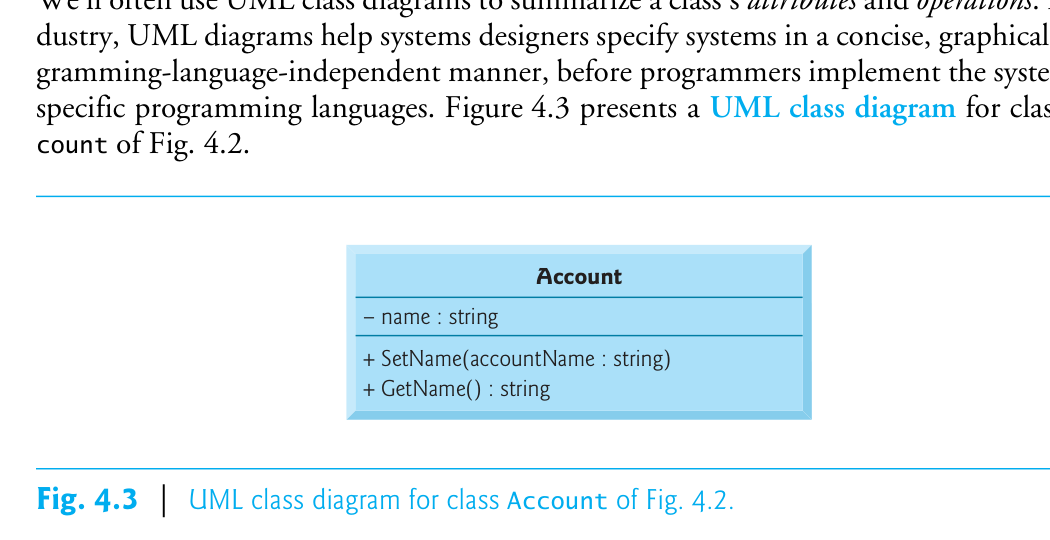
\includegraphics[width=0.95\textwidth]{images/fig4_03_uml_account.png}
      \end{center}
    \end{column}

    \begin{column}{0.50\textwidth}
      \begin{exampleblock}{\textbf{Cấu trúc 3 Ngăn của Sơ đồ Lớp UML}}
        \begin{enumerate}\small
          \item \textbf{Ngăn trên cùng (Top Compartment):}\\
          Chứa \textbf{Tên lớp} (Class Name): \texttt{Account}.
          \item \textbf{Ngăn giữa (Middle Compartment):}\\
          Chứa danh sách các \textbf{Thuộc tính / Biến thể hiện}:\\
          \texttt{- name : string}
          \begin{itemize}\footnotesize
            \item Dấu trừ (\textbf{\texttt{-}}): biểu thị chỉ định truy cập \textbf{\texttt{private}}.
            \item Theo sau là tên biến, dấu hai chấm và kiểu dữ liệu.
          \end{itemize}
          \item \textbf{Ngăn dưới cùng (Bottom Compartment):}\\
          Chứa danh sách các \textbf{Thao tác / Phương thức}:\\
          \texttt{+ SetName(accountName : string)}\\
          \texttt{+ GetName() : string}
          \begin{itemize}\footnotesize
            \item Dấu cộng (\textbf{\texttt{+}}): biểu thị chỉ định truy cập \textbf{\texttt{public}}.
            \item Kiểu trả về được đặt sau dấu hai chấm ở cuối tên phương thức.
          \end{itemize}
        \end{enumerate}
      \end{exampleblock}
    \end{column}
  \end{columns}
\end{frame}

% ==============================================================================
% SLIDE 14: QUẢN TRỊ DỰ ÁN ĐA LỚP TRONG VISUAL STUDIO
% ==============================================================================
\begin{frame}{Tổ chức Dự án Đa tệp lớp (Multiple Class Files) trong Visual Studio}
  \begin{columns}[T]
    \begin{column}{0.48\textwidth}
      \begin{block}{\textbf{Quy trình Tạo Dự án Đa tệp Lớp}}
        \begin{enumerate}\small
          \item Tạo dự án Console Application mới tên \texttt{AccountTest}.
          \item Đổi tên tệp \texttt{Program.cs} thành \texttt{AccountTest.cs} (chứa \texttt{static void Main}).
          \item Vào menu \textbf{Project} $\to$ chọn \textbf{Add Class...} (hoặc chuột phải vào Project trong Solution Explorer $\to$ Add $\to$ Class).
          \item Đặt tên tệp lớp mới là \textbf{\texttt{Account.cs}} $\to$ Bấm \textbf{Add}.
          \item Soạn thảo mã nguồn lớp \texttt{Account} trong tệp \texttt{Account.cs}.
        \end{enumerate}
      \end{block}
    \end{column}

    \begin{column}{0.48\textwidth}
      \begin{exampleblock}{\textbf{Cơ chế Liên kết trong C\# / .NET}}
        \begin{itemize}\small
          \item Trong C\#, tất cả các tệp mã nguồn (\texttt{.cs}) nằm trong cùng một Dự án (\textit{Project}) và cùng một Không gian tên (\textit{Namespace}) sẽ \textbf{tự động nhìn thấy nhau}!
          \item Lớp \texttt{AccountTest} có thể gọi trực tiếp \texttt{new Account()} mà không cần phải viết câu lệnh \texttt{\#include} như trong C++.
          \item Trình biên dịch C\# sẽ tự động gom tất cả các tệp \texttt{.cs} để biên dịch thành một tệp thực thi \texttt{.exe} duy nhất.
        \end{itemize}
      \end{exampleblock}
    \end{column}
  \end{columns}
\end{frame}

% ==============================================================================
% SLIDE 15: ĐÓNG GÓI & ẨN GIẤU DỮ LIỆU (FIG 4.4)
% ==============================================================================
\begin{frame}{Nguyên lý Đóng gói (Encapsulation) \& Ẩn giấu Dữ liệu (Hình 4.4)}
  \begin{columns}[T]
    \begin{column}{0.48\textwidth}
      \begin{center}
        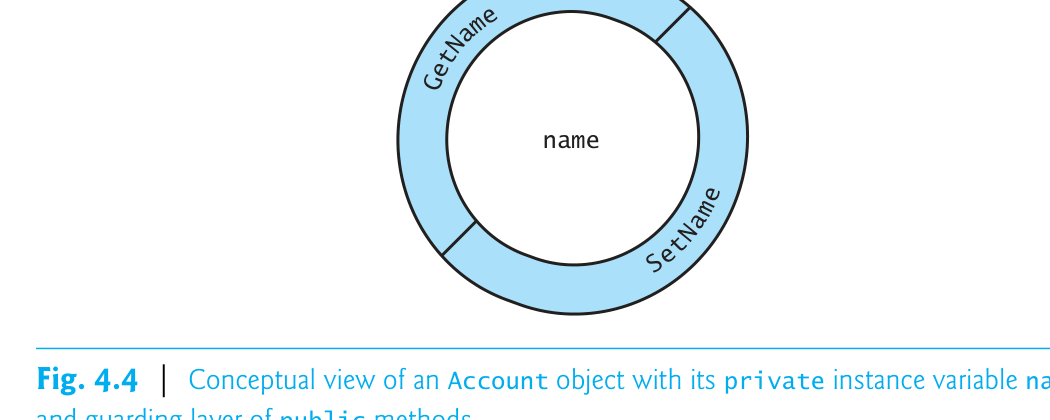
\includegraphics[width=0.95\textwidth]{images/fig4_04_conceptual_object.png}
      \end{center}
      \begin{tcolorbox}[colback=UniLightBlue!50,colframe=UniBlue,title=\textbf{Vỏ bọc Bảo vệ Dữ liệu},fonttitle=\small\bfseries]
        \small Các phương thức \texttt{public} tạo thành lớp vỏ bảo vệ (\textit{Wrapper}), ngăn chặn truy cập tùy tiện từ thế giới bên ngoài vào lõi dữ liệu \texttt{private}.
      \end{tcolorbox}
    \end{column}

    \begin{column}{0.50\textwidth}
      \begin{block}{\textbf{Lợi ích Vàng của Đóng gói (Encapsulation)}}
        \begin{itemize}\small
          \item \textbf{Ẩn giấu dữ liệu (Data Hiding):} Bên ngoài không thể gán các giá trị sai lệch hoặc phá hoại trạng thái nội bộ của đối tượng.
          \item \textbf{Toàn vẹn dữ liệu (Data Integrity):} Mọi thay đổi dữ liệu bắt buộc phải đi qua phương thức gán, nơi lập trình viên có thể chèn các câu lệnh kiểm tra tính hợp lệ (\textit{Validation}).
          \item \textbf{Dễ bảo trì (Maintainability):} Nếu cấu trúc lưu trữ nội bộ bên trong lớp thay đổi, mã nguồn của các lớp bên ngoài gọi nó hoàn toàn không bị ảnh hưởng!
        \end{itemize}
      \end{block}
    \end{column}
  \end{columns}
\end{frame}

% ==============================================================================
% SLIDE 16: CHECKPOINT 1 & LAB 1
% ==============================================================================
\begin{frame}{Checkpoint 1: Kiểm tra Nhanh \& Thực hành Tiết 1}
  \begin{columns}[T]
    \begin{column}{0.48\textwidth}
      \begin{tcolorbox}[colback=UniOrange!10,colframe=UniOrange,title=\textbf{Quiz Checkpoint 1},fonttitle=\small\bfseries]
        \small \textbf{Câu 1:} Điều gì xảy ra nếu cố truy cập biến \texttt{private name} từ lớp \texttt{AccountTest} (\texttt{myAccount.name = "Jane";})?\\
        \textbf{A.} Chạy bình thường\\
        \textbf{B.} Lỗi biên dịch: 'name is inaccessible due to its protection level' \checkmark\\
        \textbf{C.} Bị gán giá trị null\\
        \vspace{2mm}
        \textbf{Câu 2:} Giá trị mặc định của biến tham chiếu khi chưa được khởi tạo là gì?\\
        \textbf{A.} \texttt{0} \quad \textbf{B.} \texttt{""} \quad \textbf{C.} \texttt{null} \checkmark \quad \textbf{D.} \texttt{undefined}
      \end{tcolorbox}
    \end{column}

    \begin{column}{0.48\textwidth}
      \begin{tcolorbox}[colback=UniGreen!10,colframe=UniGreen,title=\textbf{Hands-on Lab 1 (15 Phút)},fonttitle=\small\bfseries]
        \begin{enumerate}\small
          \item Mở Visual Studio, tạo Solution \texttt{Chapter04\_Labs}.
          \item Tạo Project Console \texttt{AccountApp}.
          \item Viết tệp \texttt{Account.cs} với biến \texttt{private string name} và 2 phương thức \texttt{SetName}, \texttt{GetName}.
          \item Viết tệp \texttt{AccountTest.cs} chứa phương thức \texttt{Main}.
          \item Khởi tạo 2 đối tượng tài khoản khác nhau (\texttt{account1}, \texttt{account2}), gán tên và in ra màn hình.
        \end{enumerate}
      \end{tcolorbox}
    \end{column}
  \end{columns}
\end{frame}

% ==============================================================================
% SLIDE 17: TIẾT 2 DIVIDER
% ==============================================================================
\begin{frame}[plain]
  \vfill
  \centering
  \begin{beamercolorbox}[sep=8pt,center,shadow=true,rounded=true]{palette primary}
    {\Huge \textbf{TIẾT 2}}\\[2mm]
    {\Large \textbf{THUỘC TÍNH (PROPERTIES), AUTO-IMPLEMENTED PROPERTIES \& HÀM TẠO (CONSTRUCTORS)}}
  \end{beamercolorbox}
  \vfill
\end{frame}

% ==============================================================================
% SLIDE 18: GIỚI THIỆU THUỘC TÍNH C# (FIG 4.5)
% ==============================================================================
\begin{frame}[fragile]{Giới thiệu Thuộc tính (Properties) trong C\# (Hình 4.5)}
  \begin{columns}[T]
    \begin{column}{0.55\textwidth}
      \begin{tcolorbox}[colback=CodeBg,colframe=UniNavy,title=\textbf{AccountTest.cs dùng Property (Fig. 4.5)},fonttitle=\small\bfseries]
\begin{lstlisting}
// Fig. 4.5: AccountTest.cs with property
using System;

class AccountTest
{
   static void Main()
   {
      Account myAccount = new Account();

      // Read initial name using property Name
      Console.WriteLine($"Initial: {myAccount.Name}");

      Console.Write("Enter name: ");
      string theName = Console.ReadLine();
      myAccount.Name = theName; // Set property!

      // Read updated name using property Name
      Console.WriteLine($"Updated: {myAccount.Name}");
   }
}
\end{lstlisting}
      \end{tcolorbox}
    \end{column}

    \begin{column}{0.43\textwidth}
      \begin{exampleblock}{\textbf{Cú pháp Thuộc tính C\# Đột phá}}
        \begin{itemize}\small
          \item \textbf{Gán dữ liệu:}\\
          Thay vì gọi \texttt{myAccount.SetName(theName);}\\
          $\to$ Ta viết tự nhiên như gán biến:
          \texttt{myAccount.Name = theName;}
          \item \textbf{Đọc dữ liệu:}\\
          Thay vì gọi \texttt{myAccount.GetName()}\\
          $\to$ Ta truy xuất trực tiếp:
          \texttt{myAccount.Name}
          \item \textbf{Bản chất:} Nhìn bên ngoài như biến công khai (\textit{field}), nhưng bên trong thực thi như phương thức bảo vệ!
        \end{itemize}
      \end{exampleblock}
    \end{column}
  \end{columns}
\end{frame}

% ==============================================================================
% SLIDE 19: CẤU TRÚC PROPERTY NAME (FIG 4.6)
% ==============================================================================
\begin{frame}[fragile]{Cấu trúc Thuộc tính \texttt{Name}: Bộ truy cập \texttt{get} và \texttt{set} (Hình 4.6)}
  \begin{columns}[T]
    \begin{column}{0.55\textwidth}
      \begin{tcolorbox}[colback=CodeBg,colframe=UniNavy,title=\textbf{Account.cs with Property (Fig. 4.6)},fonttitle=\small\bfseries]
\begin{lstlisting}
// Fig. 4.6: Account.cs with property
class Account
{
   private string name; // backing field

   // Name property replaces SetName and GetName
   public string Name
   {
      get // get accessor
      {
         return name;
      }
      set // set accessor
      {
         name = value;
      }
   }
}
\end{lstlisting}
      \end{tcolorbox}
    \end{column}

    \begin{column}{0.43\textwidth}
      \begin{block}{\textbf{Bộ truy cập \texttt{get} (Getter)}}
        \begin{itemize}\small
          \item Tương đương phương thức \texttt{GetName()}.
          \item Thực thi tự động khi thuộc tính nằm bên \textbf{vế phải} phép gán hoặc trong lệnh in.
        \end{itemize}
      \end{block}
      \begin{exampleblock}{\textbf{Bộ truy cập \texttt{set} (Setter)}}
        \begin{itemize}\small
          \item Tương đương phương thức \texttt{SetName()}.
          \item Thực thi tự động khi thuộc tính nằm bên \textbf{vế trái} của phép gán: \texttt{myAccount.Name = "...";}.
        \end{itemize}
      \end{exampleblock}
    \end{column}
  \end{columns}
\end{frame}

% ==============================================================================
% SLIDE 20: TỪ KHÓA NGỮ CẢNH VALUE
% ==============================================================================
\begin{frame}{Từ khóa Ngữ cảnh \texttt{value} trong Bộ truy cập \texttt{set}}
  \begin{columns}[T]
    \begin{column}{0.48\textwidth}
      \begin{tcolorbox}[colback=UniLightBlue!40,colframe=UniNavy,title=\textbf{Cơ chế Hoạt động của \texttt{value}},fonttitle=\small\bfseries]
        \small Khi câu lệnh sau được thực thi:
        \begin{center}
          \texttt{myAccount.Name = "Jane Green";}
        \end{center}
        \begin{enumerate}\small
          \item Trình biên dịch C\# tự động gọi bộ truy cập \texttt{set} của thuộc tính \texttt{Name}.
          \item Giá trị vế phải (\texttt{"Jane Green"}) được truyền ngầm định vào một tham số nội bộ tên là \textbf{\texttt{value}}.
          \item Kiểu dữ liệu của \texttt{value} luôn luôn trùng khớp với kiểu dữ liệu của thuộc tính (\texttt{string}).
          \item Dòng lệnh \texttt{name = value;} sẽ cất giá trị này vào biến hậu thuẫn \texttt{name}.
        \end{enumerate}
      \end{tcolorbox}
    \end{column}

    \begin{column}{0.48\textwidth}
      \begin{block}{\textbf{Từ khóa Ngữ cảnh (Contextual Keyword) là gì?}}
        \begin{itemize}\small
          \item \texttt{value} chỉ có ý nghĩa đặc biệt bên trong khối \texttt{set} của một Thuộc tính.
          \item Ở các vị trí khác ngoài \texttt{set}, bạn vẫn có thể dùng chữ \texttt{value} để đặt tên biến bình thường (ví dụ: \texttt{int value = 10;}).
          \item Đây là thiết kế tinh tế của C\# để giữ tính tương thích mã nguồn.
        \end{itemize}
      \end{block}
      \begin{alertblock}{\textbf{Khái niệm Backing Field:}}
        Biến \texttt{private string name} được gọi là \textbf{Biến hậu thuẫn (Backing Field)} vì nó âm thầm lưu giữ dữ liệu thực tế phía sau lớp vỏ Thuộc tính \texttt{Name}.
      \end{alertblock}
    \end{column}
  \end{columns}
\end{frame}

% ==============================================================================
% SLIDE 21: SƠ ĐỒ LỚP UML VỚI PROPERTY (FIG 4.7)
% ==============================================================================
\begin{frame}{Sơ đồ lớp UML Biểu diễn Thuộc tính với Stereotype (Hình 4.7)}
  \begin{columns}[T]
    \begin{column}{0.48\textwidth}
      \begin{center}
        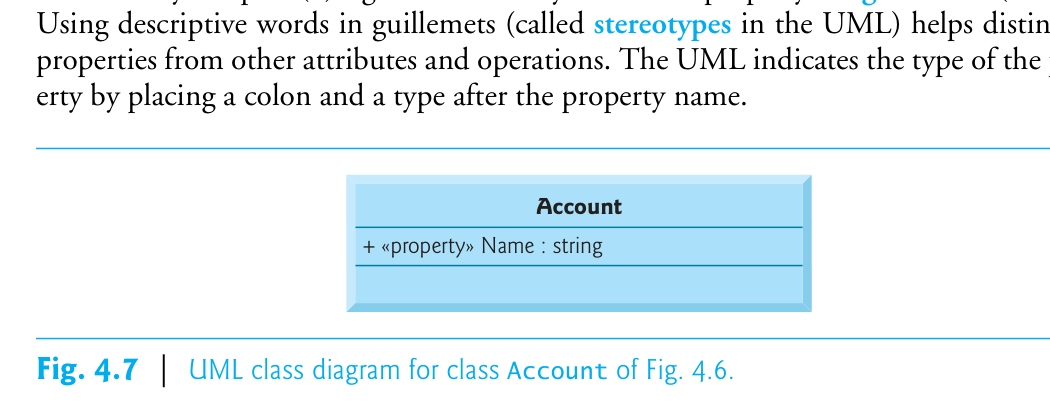
\includegraphics[width=0.95\textwidth]{images/fig4_07_uml_properties.png}
      \end{center}
    \end{column}

    \begin{column}{0.50\textwidth}
      \begin{exampleblock}{\textbf{Quy ước Biểu diễn Thuộc tính trong UML}}
        \begin{itemize}\small
          \item \textbf{Vị trí đặt:} Thuộc tính \texttt{Name} được đặt ở \textbf{Ngăn thứ 3} (ngăn Thao tác / Phương thức) của hình chữ nhật UML.
          \item \textbf{Stereotype \guillemotleft property\guillemotright:}\\
          Ký hiệu đặt trong cặp ngoặc kép Pháp \guillemotleft \dots \guillemotright\ báo hiệu đây là một \textbf{Thuộc tính} đặc trưng của C\#, chứ không phải một phương thức thông thường!
          \item \textbf{Cú pháp chuẩn:}\\
          \texttt{+ «property» Name : string}
          \begin{itemize}\footnotesize
            \item Dấu cộng (\texttt{+}): Chỉ định truy cập \texttt{public}.
            \item \texttt{Name}: Tên thuộc tính (viết hoa PascalCase).
            \item \texttt{string}: Kiểu dữ liệu của thuộc tính.
          \end{itemize}
        \end{itemize}
      \end{exampleblock}
    \end{column}
  \end{columns}
\end{frame}

% ==============================================================================
% SLIDE 22: AUTO-IMPLEMENTED PROPERTIES
% ==============================================================================
\begin{frame}[fragile]{Thuộc tính Tự động (Auto-Implemented Properties)}
  \begin{tcolorbox}[colback=CodeBg,colframe=UniNavy,title=\textbf{Cú pháp Siêu Tinh gọn của Auto-Implemented Property},fonttitle=\small\bfseries]
\begin{lstlisting}
class Account
{
   public string Name { get; set; } // Auto-implemented property!
}
\end{lstlisting}
  \end{tcolorbox}
  \begin{columns}[T]
    \begin{column}{0.48\textwidth}
      \begin{block}{\textbf{Cơ chế Sinh mã Ngầm của Trình biên dịch}}
        \begin{itemize}\small
          \item Khi viết \texttt{public string Name \{ get; set; \}}, lập trình viên \textbf{không cần khai báo biến \texttt{private string name;}}.
          \item Trình biên dịch C\# sẽ tự động tạo ra một biến hậu thuẫn ẩn danh (\textit{hidden private backing field}) trong mã máy MSIL.
          \item Trình biên dịch tự động cài đặt mã đọc/ghi cơ bản cho \texttt{get} và \texttt{set}.
        \end{itemize}
      \end{block}
    \end{column}

    \begin{column}{0.48\textwidth}
      \begin{exampleblock}{\textbf{Ưu thế Vượt trội}}
        \begin{itemize}\small
          \item Giảm từ \textbf{15 dòng code} xuống chỉ còn \textbf{đúng 1 dòng}!
          \item Mã nguồn cực kỳ gọn gàng, tăng tốc độ phát triển phần mềm gấp nhiều lần.
          \item Vẫn đảm bảo tính đóng gói: Sau này nếu cần kiểm tra tính hợp lệ (\textit{validation}), ta dễ dàng mở rộng thành thuộc tính tường minh mà không làm vỡ các mã nguồn bên ngoài!
        \end{itemize}
      \end{exampleblock}
    \end{column}
  \end{columns}
\end{frame}

% ==============================================================================
% SLIDE 23: SO SÁNH AUTO-PROPERTY VS THUỘC TÍNH CÓ BACKING FIELD
% ==============================================================================
\begin{frame}{So sánh: Thuộc tính Tự động vs Thuộc tính Tường minh}
  \begin{table}
    \centering\small
    \begin{tabularx}{\textwidth}{lXX}
      \toprule
      \textbf{Tiêu chí So sánh} & \textbf{Thuộc tính Tự động (Auto-Property)} & \textbf{Thuộc tính Tường minh (Explicit Backing Field)} \\
      \midrule
      \textbf{Cú pháp khai báo} & \texttt{public string Name \{ get; set; \}} & Khai báo biến \texttt{private} riêng + khối mã \texttt{get \{ ... \}} và \texttt{set \{ ... \}} \\
      \textbf{Biến hậu thuẫn} & Do trình biên dịch tự động sinh ngầm trong mã IL & Lập trình viên tự định nghĩa và quản lý trực tiếp \\
      \textbf{Cài đặt Logic bổ sung} & \textbf{Không thể}! Chỉ đọc và ghi đơn thuần & \textbf{Hoàn toàn có thể}: Kiểm tra tính hợp lệ (Validation), tính toán, log dữ liệu \\
      \textbf{Khi nào nên dùng?} & Khi thuộc tính chỉ đơn thuần lưu và trả giá trị không cần kiểm tra & Khi cần kiểm tra dữ liệu hợp lệ (ví dụ: số dư $> 0$, tuổi $\ge 18$) \\
      \bottomrule
    \end{tabularx}
  \end{table}
  \vspace{2mm}
  \begin{alertblock}{\textbf{Nguyên tắc Thực chiến của Kỹ sư C\#:}}
    Mặc định luôn bắt đầu bằng \textbf{Auto-Implemented Property}! Chỉ chuyển sang viết biến hậu thuẫn tường minh khi nghiệp vụ bắt đầu xuất hiện logic kiểm tra (\textit{Validation}) hoặc tính toán đặc biệt.
  \end{alertblock}
\end{frame}

% ==============================================================================
% SLIDE 24: TẠI SAO CẦN HÀM TẠO (CONSTRUCTORS)?
% ==============================================================================
\begin{frame}{Vấn đề Khởi tạo Đối tượng: Tại sao cần Hàm tạo (Constructors)?}
  \begin{columns}[T]
    \begin{column}{0.48\textwidth}
      \begin{block}{\textbf{Hạn chế của Cách làm Cũ (Hình 4.1 \& 4.5)}}
        \begin{itemize}\small
          \item Bước 1: Tạo đối tượng rỗng: \texttt{Account a = new Account();} $\to$ Biến \texttt{Name} ban đầu bị mang giá trị \textbf{\texttt{null}}!
          \item Bước 2: Phải gọi thêm lệnh gán riêng biệt: \texttt{a.Name = "Jane Green";}.
          \item \textbf{Rủi ro lớn:} Nếu lập trình viên quên bước 2, đối tượng sẽ tồn tại ở trạng thái không hoàn thiện (\textit{Incomplete/Invalid State}), rất dễ gây lỗi crash hệ thống \texttt{NullReferenceException}!
        \end{itemize}
      \end{block}
    \end{column}

    \begin{column}{0.48\textwidth}
      \begin{exampleblock}{\textbf{Giải pháp Tối ưu: Hàm tạo (Constructor)}}
        \begin{itemize}\small
          \item \textbf{Hàm tạo (Constructor)} cho phép \textbf{truyền dữ liệu khởi tạo ngay trong khoảnh khắc đối tượng được sinh ra}!
          \item Cú pháp: \texttt{Account a = new Account("Jane Green");}
          \item Đảm bảo đối tượng ngay khi bước ra khỏi dây chuyền sản xuất \texttt{new} đã ở trạng thái hợp lệ 100\% với đầy đủ thông tin ban đầu!
        \end{itemize}
      \end{exampleblock}
    \end{column}
  \end{columns}
  \vspace{2mm}
  \begin{alertblock}{\textbf{Quy luật Công nghiệp:}}
    Không bao giờ để một đối tượng ra đời ở trạng thái rỗng nếu nghiệp vụ của nó bắt buộc phải có thông tin định danh ban đầu!
  \end{alertblock}
\end{frame}

% ==============================================================================
% SLIDE 25: KHAI BÁO HÀM TẠO TRONG ACCOUNT.CS (FIG 4.8)
% ==============================================================================
\begin{frame}[fragile]{Khai báo Hàm tạo trong lớp \texttt{Account.cs} (Hình 4.8)}
  \begin{columns}[T]
    \begin{column}{0.55\textwidth}
      \begin{tcolorbox}[colback=CodeBg,colframe=UniNavy,title=\textbf{Account.cs with Constructor (Fig. 4.8)},fonttitle=\small\bfseries]
\begin{lstlisting}
// Fig. 4.8: Account.cs
class Account
{
   // Auto-implemented property
   public string Name { get; set; }

   // Constructor initializes Name with parameter
   public Account(string accountName)
   {
      Name = accountName; // sets Name property
   }
}
\end{lstlisting}
      \end{tcolorbox}
    \end{column}

    \begin{column}{0.43\textwidth}
      \begin{block}{\textbf{3 Quy tắc Vàng về Hàm tạo}}
        \begin{enumerate}\small
          \item \textbf{Tên hàm tạo:}\\
          Bắt buộc phải trùng \textbf{khớp 100\%} với tên của lớp: \texttt{Account}.
          \item \textbf{Không có kiểu trả về:}\\
          Tuyệt đối \textbf{không có kiểu trả về}, ngay cả từ khóa \texttt{void} cũng không được phép có!
          \item \textbf{Thời điểm gọi:}\\
          Được máy ảo .NET tự động kích hoạt duy nhất \textbf{một lần} ngay khi toán tử \texttt{new} cấp phát bộ nhớ xong.
        \end{enumerate}
      \end{block}
    \end{column}
  \end{columns}
\end{frame}

% ==============================================================================
% SLIDE 26: KHỞI TẠO ĐỐI TƯỢNG VỚI CONSTRUCTOR (FIG 4.9)
% ==============================================================================
\begin{frame}[fragile]{Khởi tạo nhiều Đối tượng với Đối số trong \texttt{AccountTest.cs} (Hình 4.9)}
  \begin{columns}[T]
    \begin{column}{0.55\textwidth}
      \begin{tcolorbox}[colback=CodeBg,colframe=UniNavy,title=\textbf{AccountTest.cs using Constructor (Fig. 4.9)},fonttitle=\small\bfseries]
\begin{lstlisting}
// Fig. 4.9: AccountTest.cs
using System;

class AccountTest
{
   static void Main()
   {
      // Create two Account objects using constructor
      Account account1 = new Account("Jane Green");
      Account account2 = new Account("John Blue");

      // Display initial balance of each account
      Console.WriteLine($"account1: {account1.Name}");
      Console.WriteLine($"account2: {account2.Name}");
   }
}
\end{lstlisting}
      \end{tcolorbox}
    \end{column}

    \begin{column}{0.43\textwidth}
      \begin{tcolorbox}[colback=UniDark,colframe=UniNavy,title=\textbf{Màn hình Console Output},fonttitle=\small\bfseries]
        \color{white}\ttfamily\scriptsize
        account1: Jane Green\\
        account2: John Blue
      \end{tcolorbox}
      \begin{exampleblock}{\textbf{Phân tích Kiến trúc Bộ nhớ}}
        \begin{itemize}\small
          \item Cung cấp 2 đối tượng độc lập hoàn toàn trong vùng nhớ Heap.
          \item Ô nhớ của \texttt{account1} lưu trữ giá trị \texttt{"Jane Green"}.
          \item Ô nhớ của \texttt{account2} lưu trữ giá trị \texttt{"John Blue"}.
          \item Cả hai đối tượng đều được khởi tạo sạch sẽ ngay tại dòng khai báo!
        \end{itemize}
      \end{exampleblock}
    \end{column}
  \end{columns}
\end{frame}

% ==============================================================================
% SLIDE 27: HÀM TẠO MẶC ĐỊNH VS TÙY BIẾN
% ==============================================================================
\begin{frame}{Hàm tạo Mặc định (Default Constructor) vs Hàm tạo Tùy biến}
  \begin{columns}[T]
    \begin{column}{0.48\textwidth}
      \begin{block}{\textbf{Hàm tạo Mặc định (Default Constructor)}}
        \begin{itemize}\small
          \item Nếu một lớp \textbf{không khai báo bất kỳ hàm tạo nào}, trình biên dịch C\# sẽ tự động tạo ngầm một hàm tạo mặc định \textbf{không tham số} (\textit{parameterless}).
          \item Hàm tạo mặc định này chỉ đơn giản khởi tạo các biến thể hiện về giá trị mặc định (\texttt{null}, \texttt{0}, \texttt{false}).
          \item Nhờ đó bạn mới có thể gọi: \texttt{new Account()} như ở Hình 4.1 và 4.5.
        \end{itemize}
      \end{block}
    \end{column}

    \begin{column}{0.48\textwidth}
      \begin{alertblock}{\textbf{Cạm bẫy Biên dịch Cực kỳ Quan trọng!}}
        \begin{itemize}\small
          \item Một khi bạn đã \textbf{tự tay định nghĩa ít nhất 1 hàm tạo có tham số} (như \texttt{public Account(string name)}):
          \item $\to$ Trình biên dịch C\# sẽ \textbf{NGAY LẬP TỨC XÓA BỎ} hàm tạo mặc định không tham số!
          \item Khi đó, nếu bạn gọi lệnh \texttt{new Account()} không truyền tham số, trình biên dịch sẽ \textbf{báo lỗi ngay}: \textit{CS7036: There is no argument given that corresponds to the required formal parameter}.
        \end{itemize}
      \end{alertblock}
    \end{column}
  \end{columns}
  \vspace{2mm}
  \begin{exampleblock}{\textbf{Giải pháp:}}
    Nếu muốn vừa tạo được đối tượng rỗng \texttt{new Account()} vừa tạo được đối tượng có tham số \texttt{new Account("Jane")}, bạn phải chủ động viết \textbf{cả 2 hàm tạo} (Kỹ thuật Nạp chồng hàm tạo - Constructor Overloading)!
  \end{exampleblock}
\end{frame}

% ==============================================================================
% SLIDE 28: SƠ ĐỒ LỚP UML BIỂU DIỄN CONSTRUCTOR (FIG 4.10)
% ==============================================================================
\begin{frame}{Sơ đồ lớp UML Biểu diễn Hàm tạo (Hình 4.10)}
  \begin{columns}[T]
    \begin{column}{0.48\textwidth}
      \begin{center}
        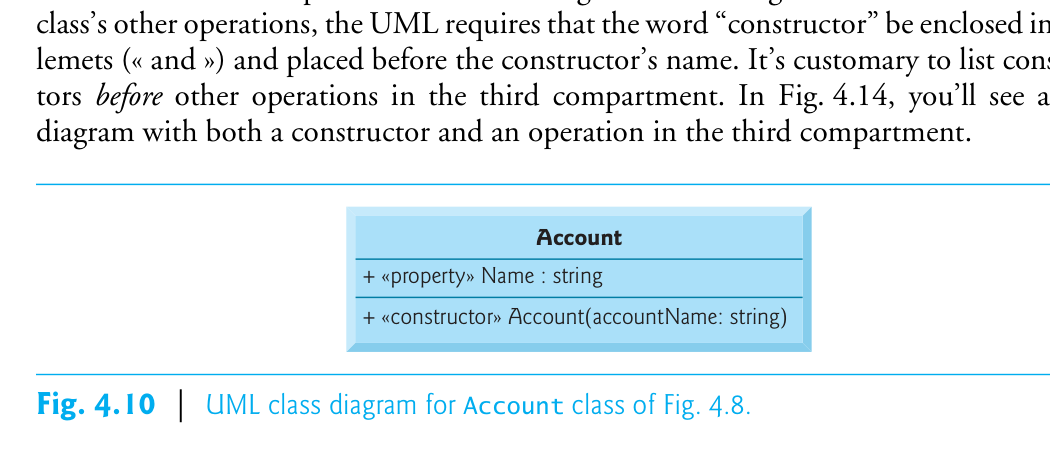
\includegraphics[width=0.95\textwidth]{images/fig4_10_uml_constructor.png}
      \end{center}
    \end{column}

    \begin{column}{0.50\textwidth}
      \begin{exampleblock}{\textbf{Quy ước Biểu diễn Hàm tạo trong UML}}
        \begin{itemize}\small
          \item \textbf{Vị trí đặt:} Được liệt kê ở \textbf{đầu tiên} trong Ngăn thứ 3 (trước tất cả các thao tác/thuộc tính thông thường).
          \item \textbf{Cú pháp chuẩn:}\\
          \texttt{+ Account(accountName : string)}
          \begin{itemize}\footnotesize
            \item Dấu cộng (\texttt{+}): Chỉ định truy cập \texttt{public}.
            \item Tên hàm tạo: Trùng hoàn toàn với tên lớp \texttt{Account}.
            \item Tham số: \texttt{accountName : string}.
            \item \textbf{Đặc biệt:} Tuyệt đối \textbf{không có kiểu trả về} ở phía sau (không có \texttt{: void} hay \texttt{: string})!
          \end{itemize}
          \item Phía dưới là thuộc tính \texttt{+ «property» Name : string}.
        \end{itemize}
      \end{exampleblock}
    \end{column}
  \end{columns}
\end{frame}

% ==============================================================================
% SLIDE 29: CHECKPOINT 2 & LAB 2
% ==============================================================================
\begin{frame}{Checkpoint 2: Kiểm tra Nhanh \& Thực hành Tiết 2}
  \begin{columns}[T]
    \begin{column}{0.48\textwidth}
      \begin{tcolorbox}[colback=UniOrange!10,colframe=UniOrange,title=\textbf{Quiz Checkpoint 2},fonttitle=\small\bfseries]
        \small \textbf{Câu 1:} Trong bộ truy cập \texttt{set}, từ khóa nào đại diện cho giá trị được truyền vào?\\
        \textbf{A.} \texttt{param} \quad \textbf{B.} \texttt{input} \quad \textbf{C.} \texttt{value} \checkmark \quad \textbf{D.} \texttt{data}\\
        \vspace{2mm}
        \textbf{Câu 2:} Sau khi khai báo hàm tạo \texttt{public Account(string name)}, lệnh \texttt{Account a = new Account();} có biên dịch được không?\\
        \textbf{A.} Được, C\# vẫn giữ hàm tạo mặc định\\
        \textbf{B.} Không! Lỗi biên dịch vì hàm tạo mặc định đã bị hủy \checkmark
      \end{tcolorbox}
    \end{column}

    \begin{column}{0.48\textwidth}
      \begin{tcolorbox}[colback=UniGreen!10,colframe=UniGreen,title=\textbf{Hands-on Lab 2 (15 Phút)},fonttitle=\small\bfseries]
        \begin{enumerate}\small
          \item Nâng cấp lớp \texttt{Account.cs}: Thay thế phương thức Set/Get bằng Auto-Property: \texttt{public string Name \{ get; set; \}}.
          \item Viết hàm tạo \texttt{public Account(string accountName)}.
          \item Viết thêm hàm tạo nạp chồng thứ hai: \texttt{public Account()} không tham số.
          \item Trong \texttt{AccountTest.cs}, kiểm thử tạo 1 đối tượng có đối số và 1 đối tượng không đối số. Chạy thử nghiệm!
        \end{enumerate}
      \end{tcolorbox}
    \end{column}
  \end{columns}
\end{frame}

% ==============================================================================
% SLIDE 30: TIẾT 3 DIVIDER
% ==============================================================================
\begin{frame}[plain]
  \vfill
  \centering
  \begin{beamercolorbox}[sep=8pt,center,shadow=true,rounded=true]{palette primary}
    {\Huge \textbf{TIẾT 3}}\\[2mm]
    {\Large \textbf{XỬ LÝ TIỀN TỆ VỚI KIỂU DECIMAL, DATA VALIDATION \& LAB TỔNG HỢP ATM}}
  \end{beamercolorbox}
  \vfill
\end{frame}

% ==============================================================================
% SLIDE 31: TẠI SAO PHẢI DÙNG DECIMAL CHO TIỀN TỆ?
% ==============================================================================
\begin{frame}{Bài toán Tài chính: Tại sao cấm dùng \texttt{double}/\texttt{float} cho Tiền tệ?}
  \begin{columns}[T]
    \begin{column}{0.48\textwidth}
      \begin{alertblock}{\textbf{Hiểm họa Sai số Dấu phẩy động (Floating-Point)}}
        \begin{itemize}\small
          \item Kiểu \texttt{double} và \texttt{float} biểu diễn số thực dưới dạng \textbf{nhị phân (cơ số 2)}.
          \item Nhiều phân số thập phân quen thuộc (như $0.1$ hay $0.01$) \textbf{không thể biểu diễn chính xác tuyệt đối} trong hệ nhị phân, dẫn đến số lẻ vô hạn tuần hoàn:
          \begin{center}
            \texttt{0.1 + 0.2 = 0.30000000000000004}
          \end{center}
          \item Trong phần mềm tài chính, ngân hàng, việc sai lệch dù chỉ 1 xu (0.01\$) tích lũy qua hàng triệu giao dịch sẽ gây thâm hụt hàng triệu USD và vi phạm pháp luật!
        \end{itemize}
      \end{alertblock}
    \end{column}

    \begin{column}{0.48\textwidth}
      \begin{exampleblock}{\textbf{Giải pháp C\#: Kiểu dữ liệu \texttt{decimal}}}
        \begin{itemize}\small
          \item Được Microsoft thiết kế \textbf{độc quyền cho các phép tính tài chính và tiền tệ}.
          \item Biểu diễn số theo \textbf{cơ số 10 (thập phân)}, loại trừ hoàn toàn sai số làm tròn của hệ nhị phân!
          \item \textbf{Quy tắc vàng của Kỹ sư C\#:} Trong mọi ứng dụng kế toán, thương mại điện tử, thanh toán và ngân hàng $\to$ \textbf{100\% bắt buộc dùng kiểu \texttt{decimal}}!
        \end{itemize}
      \end{exampleblock}
    \end{column}
  \end{columns}
\end{frame}

% ==============================================================================
% SLIDE 32: ĐẶC TÍNH KIỂU DECIMAL
% ==============================================================================
\begin{frame}{Đặc tính Kỹ thuật Kiểu \texttt{decimal} (128-bit) \& Hậu tố \texttt{m} / \texttt{M}}
  \begin{table}
    \centering\small
    \begin{tabularx}{\textwidth}{lXX}
      \toprule
      \textbf{Thông số Kỹ thuật} & \textbf{Kiểu \texttt{double}} & \textbf{Kiểu \texttt{decimal}} \\
      \midrule
      \textbf{Kích thước bộ nhớ} & 64-bit (8 bytes) & \textbf{128-bit (16 bytes)} -- dung lượng gấp đôi! \\
      \textbf{Độ chính xác} & 15 -- 17 chữ số có nghĩa & \textbf{28 -- 29 chữ số có nghĩa} (siêu chính xác) \\
      \textbf{Dải giá trị} & $\pm 5.0 \times 10^{-324}$ đến $\pm 1.7 \times 10^{308}$ & $\pm 1.0 \times 10^{-28}$ đến $\pm 7.9 \times 10^{28}$ \\
      \textbf{Hậu tố hằng số (Literal)} & \texttt{d} hoặc \texttt{D} (mặc định) & \textbf{\texttt{m} hoặc \texttt{M}} (ví dụ: \texttt{0.0m}, \texttt{150.75m}) \\
      \bottomrule
    \end{tabularx}
  \end{table}
  \vspace{2mm}
  \begin{alertblock}{\textbf{Cạm bẫy Cú pháp Hằng số:}}
    Nếu bạn viết \texttt{decimal balance = 100.50;}, trình biên dịch C\# sẽ báo lỗi ngay vì nó mặc định hiểu \texttt{100.50} là kiểu \texttt{double}! Bạn \textbf{bắt buộc phải thêm chữ m}: \texttt{decimal balance = 100.50m;}. Chữ \texttt{m} viết tắt của \textbf{Monetary / Money}!
  \end{alertblock}
\end{frame}

% ==============================================================================
% SLIDE 33: LỚP ACCOUNT NÂNG CẤP VỚI BALANCE (FIG 4.11)
% ==============================================================================
\begin{frame}[fragile]{Nâng cấp lớp \texttt{Account.cs}: Bổ sung Biến \texttt{balance} \& Thuộc tính (Hình 4.11)}
  \begin{tcolorbox}[colback=CodeBg,colframe=UniNavy,title=\textbf{Account.cs with Balance and Validation (Trích Fig. 4.11)},fonttitle=\small\bfseries]
\begin{lstlisting}
class Account
{
   public string Name { get; set; } // auto-implemented property
   private decimal balance; // backing field for Balance

   // Constructor with 2 parameters: name and initial balance
   public Account(string accountName, decimal initialBalance)
   {
      Name = accountName;
      Balance = initialBalance; // sets Balance using property validation!
   }

   public decimal Balance
   {
      get { return balance; }
      private set // only class can set directly, with validation!
      {
         if (value > 0.0m) // data validation: only positive balance allowed
         {
            balance = value;
         }
      }
   }
}
\end{lstlisting}
  \end{tcolorbox}
\end{frame}

% ==============================================================================
% SLIDE 34: DATA VALIDATION
% ==============================================================================
\begin{frame}{Cơ chế Kiểm tra Tính hợp lệ của Dữ liệu (Data Validation)}
  \begin{columns}[T]
    \begin{column}{0.48\textwidth}
      \begin{block}{\textbf{Tại sao phải Validation?}}
        \begin{itemize}\small
          \item Trong thực tế ngân hàng, số dư tài khoản khởi tạo không bao giờ được phép là số âm!
          \item Nếu người dùng truyền vào số âm (ví dụ: \texttt{-50.0m}):
          \begin{itemize}\footnotesize
            \item Câu lệnh điều kiện \texttt{if (value > 0.0m)} sẽ trả về \textbf{\texttt{false}}.
            \item Lệnh gán \texttt{balance = value;} bị bỏ qua.
            \item Biến \texttt{balance} vẫn giữ nguyên giá trị mặc định là \textbf{\texttt{0.0m}}.
          \end{itemize}
          \item Đối tượng tự bảo vệ mình không bị rơi vào trạng thái sai lệch!
        \end{itemize}
      \end{block}
    \end{column}

    \begin{column}{0.48\textwidth}
      \begin{exampleblock}{\textbf{Từ khóa \texttt{private set}}}
        \begin{itemize}\small
          \item Chú ý dòng khai báo: \texttt{private set}.
          \item \textbf{\texttt{get} là công khai (\texttt{public}):} Bất kỳ ai bên ngoài cũng có thể xem số dư: \texttt{Console.WriteLine(a.Balance);}.
          \item \textbf{\texttt{set} là riêng tư (\texttt{private}):} Mã nguồn bên ngoài \textbf{bị cấm tuyệt đối} không được tự tiện sửa số dư kiểu: \texttt{a.Balance = 1000000m;}.
          \item Mọi biến động số dư bắt buộc phải thông qua các giao dịch nghiệp vụ chính thống như \texttt{Deposit} hoặc \texttt{Withdraw}!
        \end{itemize}
      \end{exampleblock}
    \end{column}
  \end{columns}
\end{frame}

% ==============================================================================
% SLIDE 35: PHƯƠNG THỨC DEPOSIT
% ==============================================================================
\begin{frame}[fragile]{Phương thức Nghiệp vụ Ngân hàng: \texttt{Deposit(decimal depositAmount)}}
  \begin{tcolorbox}[colback=CodeBg,colframe=UniNavy,title=\textbf{Phương thức Nạp tiền Deposit (Fig. 4.11)},fonttitle=\small\bfseries]
\begin{lstlisting}
// method that deposits (adds) only a valid amount to the balance
public void Deposit(decimal depositAmount)
{
   if (depositAmount > 0.0m) // if the depositAmount is valid
   {
      balance = balance + depositAmount; // add it to the balance
   }
}
\end{lstlisting}
  \end{tcolorbox}
  \begin{columns}[T]
    \begin{column}{0.48\textwidth}
      \begin{block}{\textbf{Quy trình Nghiệp vụ Nạp tiền}}
        \begin{enumerate}\small
          \item Kiểm tra điều kiện đầu vào: \texttt{depositAmount > 0.0m}.
          \item Nếu người dùng nạp số tiền $\le 0$, phương thức bỏ qua, không cộng vào tài khoản và giữ nguyên số dư an toàn.
          \item Nếu tiền nạp hợp lệ, cộng dồn vào biến \texttt{balance}.
        \end{enumerate}
      \end{block}
    \end{column}

    \begin{column}{0.48\textwidth}
      \begin{exampleblock}{\textbf{Chuẩn mực Lập trình An toàn}}
        \begin{itemize}\small
          \item Đây là ví dụ mẫu mực về \textbf{Business Logic} nằm trong lớp nghiệp vụ.
          \item Không đẩy trách nhiệm kiểm tra dữ liệu cho giao diện người dùng, mà chính lớp đối tượng phải chịu trách nhiệm tự bảo vệ tính toàn vẹn của mình!
        \end{itemize}
      \end{exampleblock}
    \end{column}
  \end{columns}
\end{frame}

% ==============================================================================
% SLIDE 36: ACCOUNTTEST.CS PART 1 (FIG 4.12)
% ==============================================================================
\begin{frame}[fragile]{Khảo sát \texttt{AccountTest.cs}: Khởi tạo \& In Tiền tệ (Hình 4.12 -- Phần 1)}
  \begin{columns}[T]
    \begin{column}{0.55\textwidth}
      \begin{tcolorbox}[colback=CodeBg,colframe=UniNavy,title=\textbf{AccountTest.cs Part 1 (Fig. 4.12)},fonttitle=\small\bfseries]
\begin{lstlisting}
// Fig. 4.12: AccountTest.cs
using System;

class AccountTest
{
   static void Main()
   {
      Account account1 = new Account("Jane Green", 50.00m);
      Account account2 = new Account("John Blue", -7.53m);

      // Display initial balance of each object
      Console.WriteLine(
         $"{account1.Name}'s balance: {account1.Balance:C}");
      Console.WriteLine(
         $"{account2.Name}'s balance: {account2.Balance:C}");
\end{lstlisting}
      \end{tcolorbox}
    \end{column}

    \begin{column}{0.43\textwidth}
      \begin{tcolorbox}[colback=UniDark,colframe=UniNavy,title=\textbf{Output Khởi tạo},fonttitle=\small\bfseries]
        \color{white}\ttfamily\scriptsize
        Jane Green's balance: \$50.00\\
        John Blue's balance: \$0.00
      \end{tcolorbox}
      \begin{alertblock}{\textbf{Hiệu quả của Validation:}}
        \small \texttt{account2} được khởi tạo với số dư âm \texttt{-7.53m}, nhưng nhờ cơ chế validation trong \texttt{Balance}, số dư khởi tạo không bị âm mà được giữ an toàn ở mức \textbf{\$0.00}!
      \end{alertblock}
      \begin{exampleblock}{\textbf{Ký tự \texttt{:C} kỳ diệu:}}
        \small Cú pháp \texttt{\{account1.Balance:C\}} tự động định dạng con số \texttt{50} thành chuỗi tiền tệ \textbf{\texttt{\$50.00}} kèm dấu phân cách!
      \end{exampleblock}
    \end{column}
  \end{columns}
\end{frame}

% ==============================================================================
% SLIDE 37: ACCOUNTTEST.CS PART 2 (FIG 4.12)
% ==============================================================================
\begin{frame}[fragile]{Khảo sát \texttt{AccountTest.cs}: Nạp tiền \& Cập nhật Số dư (Hình 4.12 -- Phần 2)}
  \begin{columns}[T]
    \begin{column}{0.55\textwidth}
      \begin{tcolorbox}[colback=CodeBg,colframe=UniNavy,title=\textbf{AccountTest.cs Part 2 (Fig. 4.12)},fonttitle=\small\bfseries]
\begin{lstlisting}
      // Prompt and deposit for account1
      Console.Write("\nEnter deposit amount for account1: ");
      decimal depositAmount = 
         decimal.Parse(Console.ReadLine());
      Console.WriteLine(
         $"adding {depositAmount:C} to account1 balance\n");
      account1.Deposit(depositAmount); // deposit to account1

      // Display updated balances
      Console.WriteLine(
         $"{account1.Name}'s balance: {account1.Balance:C}");
      Console.WriteLine(
         $"{account2.Name}'s balance: {account2.Balance:C}");
   }
}
\end{lstlisting}
      \end{tcolorbox}
    \end{column}

    \begin{column}{0.43\textwidth}
      \begin{tcolorbox}[colback=UniDark,colframe=UniNavy,title=\textbf{Output Thực thi Giao dịch},fonttitle=\small\bfseries]
        \color{white}\ttfamily\scriptsize
        Enter deposit amount for account1: 25.53\\
        adding \$25.53 to account1 balance\\[2mm]
        Jane Green's balance: \$75.53\\
        John Blue's balance: \$0.00
      \end{tcolorbox}
      \begin{block}{\textbf{Lệnh \texttt{decimal.Parse}}}
        \small Tương tự \texttt{int.Parse}, phương thức \texttt{decimal.Parse} phân tích chuỗi người dùng nhập thành số thực \texttt{decimal} chính xác cao để thực hiện phép cộng số dư!
      \end{block}
    \end{column}
  \end{columns}
\end{frame}

% ==============================================================================
% SLIDE 38: ĐỊNH DẠNG TIỀN TỆ :C
% ==============================================================================
\begin{frame}{Kỹ thuật Định dạng Tiền tệ với Ký tự \texttt{:C} (Currency Format)}
  \begin{columns}[T]
    \begin{column}{0.48\textwidth}
      \begin{tcolorbox}[colback=UniLightBlue!40,colframe=UniNavy,title=\textbf{Cú pháp Định dạng Chuỗi Nội suy},fonttitle=\small\bfseries]
        \begin{center}
          \Large \texttt{\$\{biến:ký\_tự\_định\_dạng\}}
        \end{center}
        \small Ví dụ:
        \texttt{\$\{account1.Balance:C\}}
        \begin{itemize}\small
          \item Dấu hai chấm (\textbf{\texttt{:}}) phân cách giữa tên biến/biểu thức và mẫu định dạng.
          \item Ký tự \textbf{\texttt{C}} (viết tắt của \textit{Currency}): Định dạng số thành giá trị tiền tệ.
          \item Tự động thêm ký hiệu tiền tệ (\$, \texteuro, \textyen, \dots), dấu phân cách hàng nghìn (dấu phẩy hoặc dấu chấm), và 2 chữ số phần thập phân.
        \end{itemize}
      \end{tcolorbox}
    \end{column}

    \begin{column}{0.48\textwidth}
      \begin{exampleblock}{\textbf{Đa văn hóa \& Ngôn ngữ (Localization - Culture)}}
        \begin{itemize}\small
          \item Ký tự \texttt{:C} hoàn toàn phụ thuộc vào \textbf{Cài đặt Khu vực (Regional Settings / Culture)} của Hệ điều hành nơi chương trình đang chạy:
          \begin{itemize}\footnotesize
            \item Máy cài Culture \texttt{en-US} (Mỹ): Xuất \texttt{\$75.53}
            \item Máy cài Culture \texttt{vi-VN} (Việt Nam): Xuất \texttt{75,53 \textsubscript{₫}}
            \item Máy cài Culture \texttt{fr-FR} (Pháp): Xuất \texttt{75,53 \texteuro}
          \end{itemize}
          \item Tính năng này giúp phần mềm của các em tự động chuẩn hóa quốc tế mà không cần viết lại mã nguồn!
        \end{itemize}
      \end{exampleblock}
    \end{column}
  \end{columns}
\end{frame}

% ==============================================================================
% SLIDE 39: BẢNG KÝ TỰ ĐỊNH DẠNG CHUỖI (FIG 4.13)
% ==============================================================================
\begin{frame}{Bảng Tra cứu Ký tự Định dạng Chuỗi Thông dụng trong .NET (Hình 4.13)}
  \begin{table}
    \centering\small
    \begin{tabularx}{\textwidth}{llXl}
      \toprule
      \textbf{Ký tự} & \textbf{Tên Định dạng} & \textbf{Ý nghĩa \& Mô tả Chức năng} & \textbf{Ví dụ Kết quả} \\
      \midrule
      \textbf{\texttt{C}} hoặc \texttt{c} & Currency & Định dạng tiền tệ với ký hiệu tiền tệ và 2 chữ số thập phân & \texttt{123.45:C} $\to$ \textbf{\$123.45} \\
      \textbf{\texttt{D}} hoặc \texttt{d} & Decimal (Integer) & Định dạng số nguyên với số lượng chữ số tối thiểu (\texttt{D5}) & \texttt{25:D5} $\to$ \textbf{00025} \\
      \textbf{\texttt{E}} hoặc \texttt{e} & Scientific & Biểu diễn số dưới dạng ký hiệu khoa học số mũ ($e$) & \texttt{12345:E} $\to$ \textbf{1.234500E+004} \\
      \textbf{\texttt{F}} hoặc \texttt{f} & Fixed-point & Số có dấu phẩy cố định với số chữ số thập phân chỉ định & \texttt{12.3:F2} $\to$ \textbf{12.30} \\
      \textbf{\texttt{G}} hoặc \texttt{g} & General & Tự động chọn giữa Fixed-point và Scientific dạng ngắn nhất & \texttt{123.45:G} $\to$ \textbf{123.45} \\
      \textbf{\texttt{N}} hoặc \texttt{n} & Number & Định dạng số cơ bản có dấu phân cách hàng nghìn & \texttt{1234567:N2} $\to$ \textbf{1,234,567.00} \\
      \textbf{\texttt{P}} hoặc \texttt{p} & Percent & Tự động nhân 100 và thêm ký hiệu phần trăm (\%) & \texttt{0.125:P} $\to$ \textbf{12.50\%} \\
      \bottomrule
    \end{tabularx}
  \end{table}
  \vspace{-1mm}
  \begin{center}
    \footnotesize \textit{Bảng tra cứu chuẩn theo Hình 4.13 Giáo trình Visual C\# How to Program (Deitel \& Deitel).}
  \end{center}
\end{frame}

% ==============================================================================
% SLIDE 40: SƠ ĐỒ LỚP UML TOÀN DIỆN CHO ACCOUNT (FIG 4.14)
% ==============================================================================
\begin{frame}{Sơ đồ lớp UML Toàn diện của Lớp \texttt{Account} Hoàn chỉnh (Hình 4.14)}
  \begin{columns}[T]
    \begin{column}{0.48\textwidth}
      \begin{center}
        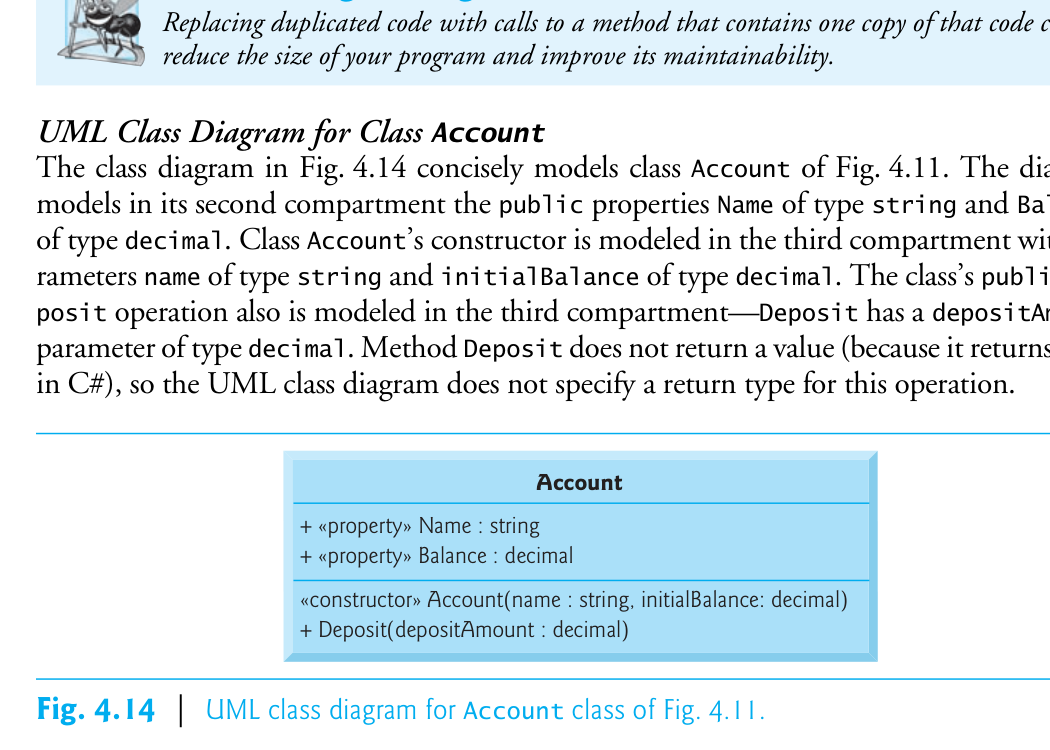
\includegraphics[width=0.95\textwidth]{images/fig4_14_uml_balance.png}
      \end{center}
    \end{column}

    \begin{column}{0.50\textwidth}
      \begin{exampleblock}{\textbf{Phân tích Sơ đồ UML Hoàn chỉnh}}
        \begin{itemize}\small
          \item \textbf{Ngăn 1:} Tên lớp \texttt{Account}.
          \item \textbf{Ngăn 2 (Attributes):}
          \begin{itemize}\footnotesize
            \item \texttt{- balance : decimal} (biến hậu thuẫn \texttt{private}).
          \end{itemize}
          \item \textbf{Ngăn 3 (Operations \& Properties):}
          \begin{itemize}\footnotesize
            \item \texttt{+ Account(accountName : string, initialBalance : decimal)} (hàm tạo 2 tham số).
            \item \texttt{+ «property» Name : string} (thuộc tính đọc/ghi).
            \item \texttt{+ «property» Balance : decimal \{readOnly\}} (chỉ đọc đối với bên ngoài).
            \item \texttt{+ Deposit(depositAmount : decimal)} (phương thức nạp tiền).
          \end{itemize}
        \end{itemize}
      \end{exampleblock}
      \begin{alertblock}{\textbf{Ký hiệu \texttt{\{readOnly\}}:}}
        \small Biểu thị thuộc tính chỉ cho phép đọc (\texttt{get}), vì bộ truy cập \texttt{set} đã được ẩn danh nội bộ (\texttt{private set}).
      \end{alertblock}
    \end{column}
  \end{columns}
\end{frame}

% ==============================================================================
% SLIDE 41: CÁC LỖI LẬP TRÌNH KINH ĐIỂN TRONG OOP C#
% ==============================================================================
\begin{frame}[fragile]{Các Lỗi Lập trình Kinh điển Cần Tránh trong OOP C\#}
  \begin{columns}[T]
    \begin{column}{0.48\textwidth}
      \begin{alertblock}{\textbf{1. Lỗi NullReferenceException}}
        \small Khai báo biến tham chiếu mà quên khởi tạo đối tượng bằng toán tử \texttt{new}:
        \begin{lstlisting}[numbers=none]
Account acc; // acc dang mang gia tri null!
acc.Deposit(100m); // CRASH chuong trinh!
        \end{lstlisting}
      \end{alertblock}
      \begin{alertblock}{\textbf{2. Lỗi Quên Hậu tố 'm' cho decimal}}
        \small Viết hằng số thập phân mà không có chữ \texttt{m}:
        \begin{lstlisting}[numbers=none]
decimal money = 50.0; // LOI BIEN DICH!
// Phai viet: 50.0m
        \end{lstlisting}
      \end{alertblock}
    \end{column}

    \begin{column}{0.48\textwidth}
      \begin{alertblock}{\textbf{3. Bẫy Đệ quy Vô hạn trong Property}}
        \small Trong \texttt{get}/\texttt{set}, gọi chính tên thuộc tính thay vì biến hậu thuẫn:
        \begin{lstlisting}[numbers=none]
public string Name {
   get { return Name; } // STACK OVERFLOW!
   set { Name = value; } // STACK OVERFLOW!
}
// Phai viet: return name; va name = value;
        \end{lstlisting}
      \end{alertblock}
      \begin{alertblock}{\textbf{4. Thêm kiểu trả về cho Hàm tạo}}
        \small Khai báo \texttt{public void Account(...) \{...\}} biến hàm tạo thành phương thức thông thường, làm mất chức năng khởi tạo!
      \end{alertblock}
    \end{column}
  \end{columns}
\end{frame}

% ==============================================================================
% SLIDE 42: TÁI CẤU TRÚC DISPLAYACCOUNT (EX 4.13)
% ==============================================================================
\begin{frame}[fragile]{Tái cấu trúc Mã nguồn: Phương thức Dùng chung \texttt{DisplayAccount} (Ex 4.13)}
  \begin{columns}[T]
    \begin{column}{0.48\textwidth}
      \begin{alertblock}{\textbf{Vấn đề: Trùng lặp Mã nguồn (Code Duplication)}}
        Trong \texttt{AccountTest.cs} (Hình 4.12), các câu lệnh in tên và số dư tài khoản bị lặp đi lặp lại tới 3 lần!
        \begin{itemize}\small
          \item Vi phạm nguyên lý vàng: \textbf{DRY -- Don't Repeat Yourself}.
          \item Nếu sau này muốn đổi cách hiển thị, ta phải sửa mã nguồn ở nhiều nơi, rất dễ bỏ sót và phát sinh lỗi.
        \end{itemize}
      \end{alertblock}
    \end{column}

    \begin{column}{0.48\textwidth}
      \begin{exampleblock}{\textbf{Giải pháp: Viết Phương thức Tái sử dụng}}
\begin{lstlisting}
// Reusable method for displaying account info
static void DisplayAccount(Account accountToDisplay)
{
   Console.WriteLine(
      $"{accountToDisplay.Name}'s balance: " +
      $"{accountToDisplay.Balance:C}");
}
\end{lstlisting}
        \small Khi cần in, chỉ việc gọi ngắn gọn:\\
        \texttt{DisplayAccount(account1);}\\
        \texttt{DisplayAccount(account2);}
      \end{exampleblock}
    \end{column}
  \end{columns}
  \vspace{2mm}
  \begin{block}{\textbf{Bài học Kỹ thuật Phần mềm:}}
    Mỗi khi thấy một đoạn mã được sao chép từ 2 lần trở lên, hãy lập tức gom nó thành một phương thức dùng chung!
  \end{block}
\end{frame}

% ==============================================================================
% SLIDE 43: MỞ RỘNG NGHIỆP VỤ: RÚT TIỀN WITHDRAW (EX 4.11)
% ==============================================================================
\begin{frame}[fragile]{Mở rộng Nghiệp vụ: Thiết kế Phương thức Rút tiền \texttt{Withdraw} (Ex 4.11)}
  \begin{tcolorbox}[colback=CodeBg,colframe=UniNavy,title=\textbf{Phương thức Rút tiền An toàn trong Account.cs},fonttitle=\small\bfseries]
\begin{lstlisting}
// Method that withdraws money if amount does not exceed balance
public void Withdraw(decimal withdrawalAmount)
{
   if (withdrawalAmount > balance)
   {
      Console.WriteLine("Withdrawal amount exceeded account balance.");
   }
   else if (withdrawalAmount > 0.0m)
   {
      balance = balance - withdrawalAmount; // deduct from balance
   }
}
\end{lstlisting}
  \end{tcolorbox}
  \begin{columns}[T]
    \begin{column}{0.48\textwidth}
      \begin{block}{\textbf{3 Kịch bản Xử lý Nghiệp vụ}}
        \begin{enumerate}\small
          \item \textbf{Kịch bản 1: Rút quá số dư}\\
          \texttt{withdrawalAmount > balance} $\to$ Báo lỗi thấu chi, không trừ tiền!
          \item \textbf{Kịch bản 2: Số tiền rút hợp lệ}\\
          \texttt{0 < withdrawalAmount <= balance} $\to$ Trừ tiền thành công.
          \item \textbf{Kịch bản 3: Số tiền rút âm hoặc 0} $\to$ Bỏ qua.
        \end{enumerate}
      \end{block}
    \end{column}

    \begin{column}{0.48\textwidth}
      \begin{exampleblock}{\textbf{Tư duy Kiến trúc sư Hệ thống}}
        \begin{itemize}\small
          \item Lớp \texttt{Account} trở thành một mô đun tự trị hoàn chỉnh.
          \item Bảo vệ số dư tài khoản không bao giờ bị âm dưới mọi tình huống vận hành!
        \end{itemize}
      \end{exampleblock}
    \end{column}
  \end{columns}
\end{frame}

% ==============================================================================
% SLIDE 44: HANDS-ON LAB 3: MINI ATM SYSTEM
% ==============================================================================
\begin{frame}{[HANDS-ON LAB 3] Xây dựng Hệ thống ATM Quản lý Tài khoản (25 Phút)}
  \begin{tcolorbox}[colback=UniGreen!10,colframe=UniGreen,title=\textbf{Nhiệm vụ Thực hành Phòng máy IT26M: Xây dựng Mini ATM App},fonttitle=\small\bfseries]
    \small Sinh viên mở Visual Studio và phát triển hoàn chỉnh dự án \textbf{\texttt{MiniATMSystem}}:
    \begin{enumerate}\small
      \item \textbf{Xây dựng lớp \texttt{Account.cs}:}
      \begin{itemize}\footnotesize
        \item Auto-property: \texttt{public string Name \{ get; set; \}}
        \item Biến hậu thuẫn: \texttt{private decimal balance;}
        \item Property \texttt{Balance} với \texttt{get} công khai và \texttt{private set} (validation $> 0.0m$).
        \item Hàm tạo 2 tham số: \texttt{Account(string name, decimal initialBalance)}.
        \item Phương thức nạp tiền: \texttt{public void Deposit(decimal amount)}.
        \item Phương thức rút tiền: \texttt{public void Withdraw(decimal amount)} (có kiểm tra thấu chi).
      \end{itemize}
      \item \textbf{Xây dựng lớp điều khiển \texttt{ATMDriver.cs}:}
      \begin{itemize}\footnotesize
        \item Viết phương thức dùng chung \texttt{static void DisplayAccount(Account acc)}.
        \item Khởi tạo 2 tài khoản: \texttt{acc1} (\$150.00) và \texttt{acc2} (\$500.00).
        \item Cho phép người dùng nhập số tiền nạp và số tiền rút từ bàn phím.
        \item Kiểm thử kịch bản rút tiền vượt quá số dư để đảm bảo thông báo cảnh báo hiển thị chính xác!
      \end{itemize}
    \end{enumerate}
  \end{tcolorbox}
\end{frame}

% ==============================================================================
% SLIDE 45: TỔNG KẾT & DẶN DÒ
% ==============================================================================
\begin{frame}{Tổng kết 5 Chuẩn đầu ra (CLOs) \& Chuẩn bị Chương 5}
  \begin{columns}[T]
    \begin{column}{0.55\textwidth}
      \begin{block}{\textbf{Bảng Checklist Chuẩn đầu ra Buổi học Chương 4}}
        \begin{itemize}\small
          \item[\checkmark] \textbf{CLO 4.1:} Nắm vững bản chất Lớp, Đối tượng, Driver Class, toán tử \texttt{new} và kiểu tham chiếu.
          \item[\checkmark] \textbf{CLO 4.2:} Thành thạo phương thức, biến thể hiện, biến cục bộ và nguyên lý Đóng gói \texttt{private}.
          \item[\checkmark] \textbf{CLO 4.3:} Sử dụng thành thạo Properties, Auto-properties \texttt{\{get; set;\}} và đọc sơ đồ lớp UML.
          \item[\checkmark] \textbf{CLO 4.4:} Khởi tạo đối tượng bằng Hàm tạo (Constructors) chuẩn mực và nạp chồng hàm tạo.
          \item[\checkmark] \textbf{CLO 4.5:} Vận dụng kiểu \texttt{decimal}, kiểm tra tính hợp lệ dữ liệu và định dạng tiền tệ \texttt{:C}.
        \end{itemize}
      \end{block}
    \end{column}

    \begin{column}{0.43\textwidth}
      \begin{exampleblock}{\textbf{Nhiệm vụ Tự học Về nhà}}
        \begin{enumerate}\small
          \item Hoàn thành bài tập lớn: \textbf{Ex 4.11 (Withdraw)}, \textbf{Ex 4.12 (Invoice Class)}, \textbf{Ex 4.13 (DisplayAccount)}.
          \item Làm 40 câu trắc nghiệm chuẩn hóa trên Cổng học tập trực tuyến.
          \item Đọc trước \textbf{Chương 5: Control Statements: Part 1} (Cấu trúc điều khiển: if, if-else, while).
        \end{enumerate}
      \end{exampleblock}
      \begin{center}
        \footnotesize \textbf{Chúc các em học tập xuất sắc và làm chủ OOP C\#!}
      \end{center}
    \end{column}
  \end{columns}
\end{frame}

\end{document}
